\section{Datenmodelle}

\subsection{DatasourceDefinition}

Für das Data-Lake-System muss eine Modellierung entwickelt werden, mit der alle Datenquellen dargestellt werden können.
Das entwickelt Modell definiert eine Datenquelle und bekommt den Namne DatasourceDefinition (deutsch: Datenquellendefinition).
Da Apache Spark verwendet wird, ist einer der wichtigsten Punkte zur definition einer Datenquelle die Erfassung der Informationen, die in Spark benötigt werden.
Dazu gehören: \begin{itemize}
    \item extra Abhängigkeiten für Spark (spark.jars.packages)
    \item das Format und Optionen für die Reader
    \item und bei benutzerdefinierten Speichern das Format, die Optionen und einen Schreibmodus für die Writer
\end{itemize}
Neben den Spark spezfischen werden noch folgende weiter Informationen erfasst: \begin{itemize}
    \item ein Name für die Datenquelle
    \item die Id einer anderen Datenquelle, falls die aktuelle eine Updatequelle ist
    \item Datum der Erstellung und letzten Änderung
    \item den Namen der Id-Spalte in den Daten (wird später für die Deltaberechnung benötigt)
    \item den Typ, der zu lesenden Daten
    \item bei Datei-Ingestions eine Liste der zu laden Dateien
    \item den Typ, wie die Daten geschrieben werden müssen
    \item eine Liste mit der Zeitsteuerung für eine kontinuierliche Ingestion
    \item eine Liste mit Plugindateien
    \item und eine Liste mit Abhängigkeiten der Plugins
\end{itemize}

Die Lese-Typen ergeben sich aus der Betrachtung, wie die Daten in das Data-Lake-System gelangen und welche Struktur sie haben.
Bei einer Pull-Ingestion ist das System dafür verantwortlich Daten aus einer Quelle zu laden.
Dies ist zum Beispiel bei Datenbanken der Fall.
Das Gegenteil dazu ist eine Push-Ingestion, bei der die Daten direkt an den Data Lake gesendet werden.
Diese muss jedoch nochmal in zwei unterschiedliche Typen unterteilt werden.
Bei einer Stream-Ingestion, also bei Datenströmen, werden kontinuierlich neue Daten an das System gesendet werden.
Und bei einer File-Ingestion werden Dateien hochgeladen, die die Daten enthalten, wobei wichtig ist, dass alle Dateien das gleiche Dateiformat haben.
Die Dateien können sich noch einmal und Daten- und Quelldatein unterscheiden.
Daten-Dateien enthalten unstrukturierte Daten und werden einfach im HDFS mit abgelegt ohne weiter verarbeitet zu werden.
Das könnten zum Beispiel Bilder oder Videos sein.
Quelldateien enthalten mindestens semistrukturierte Daten und dienen dem Zweck, in ein anderes Speicherformat, wie zum Beispiel Parquet oder eine Delta Tabelle geschrieben zu werden.
Es ist nicht möglich Daten direkt an die API zu senden.
Alle Push-Ingestions sollen über diese beiden Typen abgebildet werden.

Die Schreib-Typen kommen von den drei Optionen wo Daten abgelegt werden können.
Custom bedeutet, dass der in der DatasourceDefinition konfigurierte Speicher verwendet werden soll.
Delta ist das Speichern im internen Speicher aber mit einer Versionierung und Default ist das Speichern ohne Versionierung.

Für die Umsetzung einer unkomplizierten Versionierung werden alle veränderlichen Informationen einer DatasourceDefinition in Revisionen gespeichert.
Das betrifft alle oben genannten Felder.
Die Revisionen einer DatasourceDefinition erhalten eine fortlaufende Nummer.
Die DatasourceDefinition selbst hält dann nur noch eine Liste aller Revisionen und die Nummer der aktuellen.

\subsection{IngestionEvent}

Auch für den Zustand einer Ingestion musss ein Modell entwickelt werden.
Die Auführungen der Ingestions werden hier IngestionEvent geannant.
Dieses enthält wie die Revision eine fortlaufende Nummer, ein Start- und Enddatum, den aktuellen Status indem es befindet, die Nummer der Revision mit der es gestartet wurde und eine Fehlernachricht.

Das IngestionEvent kann auch an die DatasourceDefinition mit angehangen werden.
Dafür werden Felder hinzugefügt, die alle IngestionEvents, die Nummer des letzten und die Nummer des letzten erfolgreichen IngestionEvents enthalten.

\begin{figure}
    \centering
    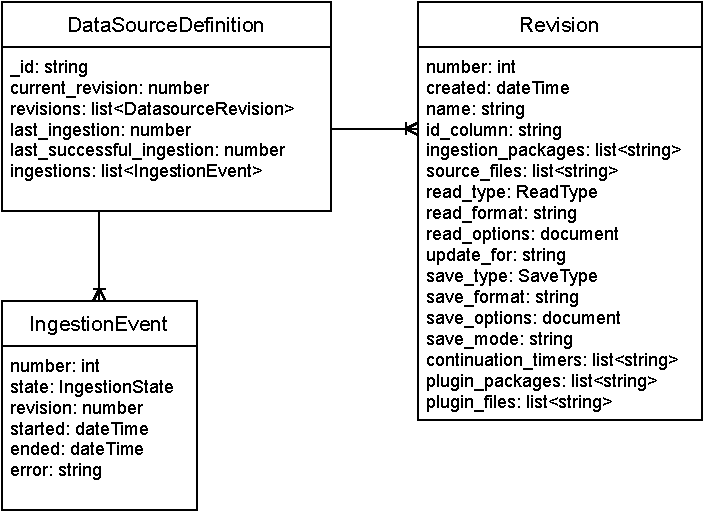
\includegraphics{Grafiken/Entwicklung-Datenmodell.pdf}
    \caption{Übersicht Datenmodell}
    \label{fig:datenmodell}
\end{figure}